\chapter{النموذج والإجراء وحزمة النماذج}
\label{ch:03-compare}

\section{ما الفرق بينها؟}
\label{sec:compare-what}

تتشابه هذه الأسماء لأنها تعمل معاً، لكن لكل منها وظيفة واحدة. فالنموذج يجمع إجابة، وحزمة النماذج ترتب عدة نماذج في مهمة واحدة، والإجراء ينفذ خطوات أو يوثّقها. وإذا عرفت ما يجب أن يحدث، عرفت الأداة التي تحتاجها.

\begin{table}[H]
\centering
\caption{المقارنة السريعة}
\label{tab:compare-quick}
\begin{tabularx}{\linewidth}{R{2.6cm} Y Y Y}
\rcHeaderRow
\thh{السؤال} & \thh{النموذج} & \thh{حزمة النماذج} & \thh{الإجراء}\\
ما وظيفته؟ & يجمع إجابة واحدة ويسير بها في مسارها. & يرتب نماذج منشورة في مهمة واحدة لكل سجل. & ينفذ خطوات آلية، أو يوثّق طريقة العمل.\\
من يعمل فيه؟ & شخص يعبّئ، ومراجِع إن وُجدت موافقة. & مكلَّف واحد أو أكثر عبر خطة تكليف. & النظام في الأتمتة، والموظفون في بطاقة الدليل.\\
كيف يبدأ؟ & بطلب جديد أو بتكليف. & بخطة تكليف فقط. & بحدث أو جدول أو تشغيل يدوي.\\
ما النتيجة؟ & ردّ له حالة، وقد يكتب إلى سجل. & تقدم موحّد، ولكل وحدة ردّها الخاص. & مهام وإشعارات وتحديثات، أو بطاقة منشورة.\\
مثال الواحة & كشف «فرن السنابل». & جولة كشف تتبعها متابعة. & مهمة لخالد بعد كل رفض.\\
\end{tabularx}
\end{table}

\begin{rcnote}[مثال: مديرية الواحة]
تعبّئ ليلى كشف «فرن السنابل»، وهذا \textbf{نموذج}. وتريد المديرية جولة فصلية فيها كشف ثم متابعة للمخالفات، وهذه \textbf{حزمة}. وبعد كل رفض تُنشأ مهمة لخالد تلقائياً، وهذا \textbf{إجراء}.
\end{rcnote}

\begin{figure}[H]
\centering
\begin{tikzpicture}[node distance=0.5cm]
\node[stepBox] (a) {\RL{هل تجمع إجابة من شخص؟\\ابدأ بنموذج}};
\node[stepBox,below=of a] (b) {\RL{هل تتكرر عدة نماذج\\على السجل نفسه؟ أنشئ حزمة}};
\node[stepBox,below=of b] (c) {\RL{هل يلزم تكليف كثيرين؟\\أنشئ خطة تكليف}};
\node[stepBox,below=of c] (d) {\RL{هل يحدث شيء تلقائياً بعد ذلك؟\\أضف إجراءً مؤتمتاً}};
\draw[flowsTo] (a) -- (b);
\draw[flowsTo] (b) -- (c);
\draw[flowsTo] (c) -- (d);
\end{tikzpicture}
\rclegend
\caption{كيف تختار؟}
\label{fig:compare-choose}
\shotnote{يبدأ المخطط بأصغر أداة تكفي العمل، ويضيف غيرها عند الحاجة فقط. فالنموذج أساس كل ما بعده: لا تضم الحزمة إلا نماذج منشورة، ولا يعمل التكليف بلا نموذج أو حزمة. ولذلك أنهِ النموذج وجرّبه قبل أن تبني فوقه.}
\end{figure}

\begin{figure}[H]
\centering
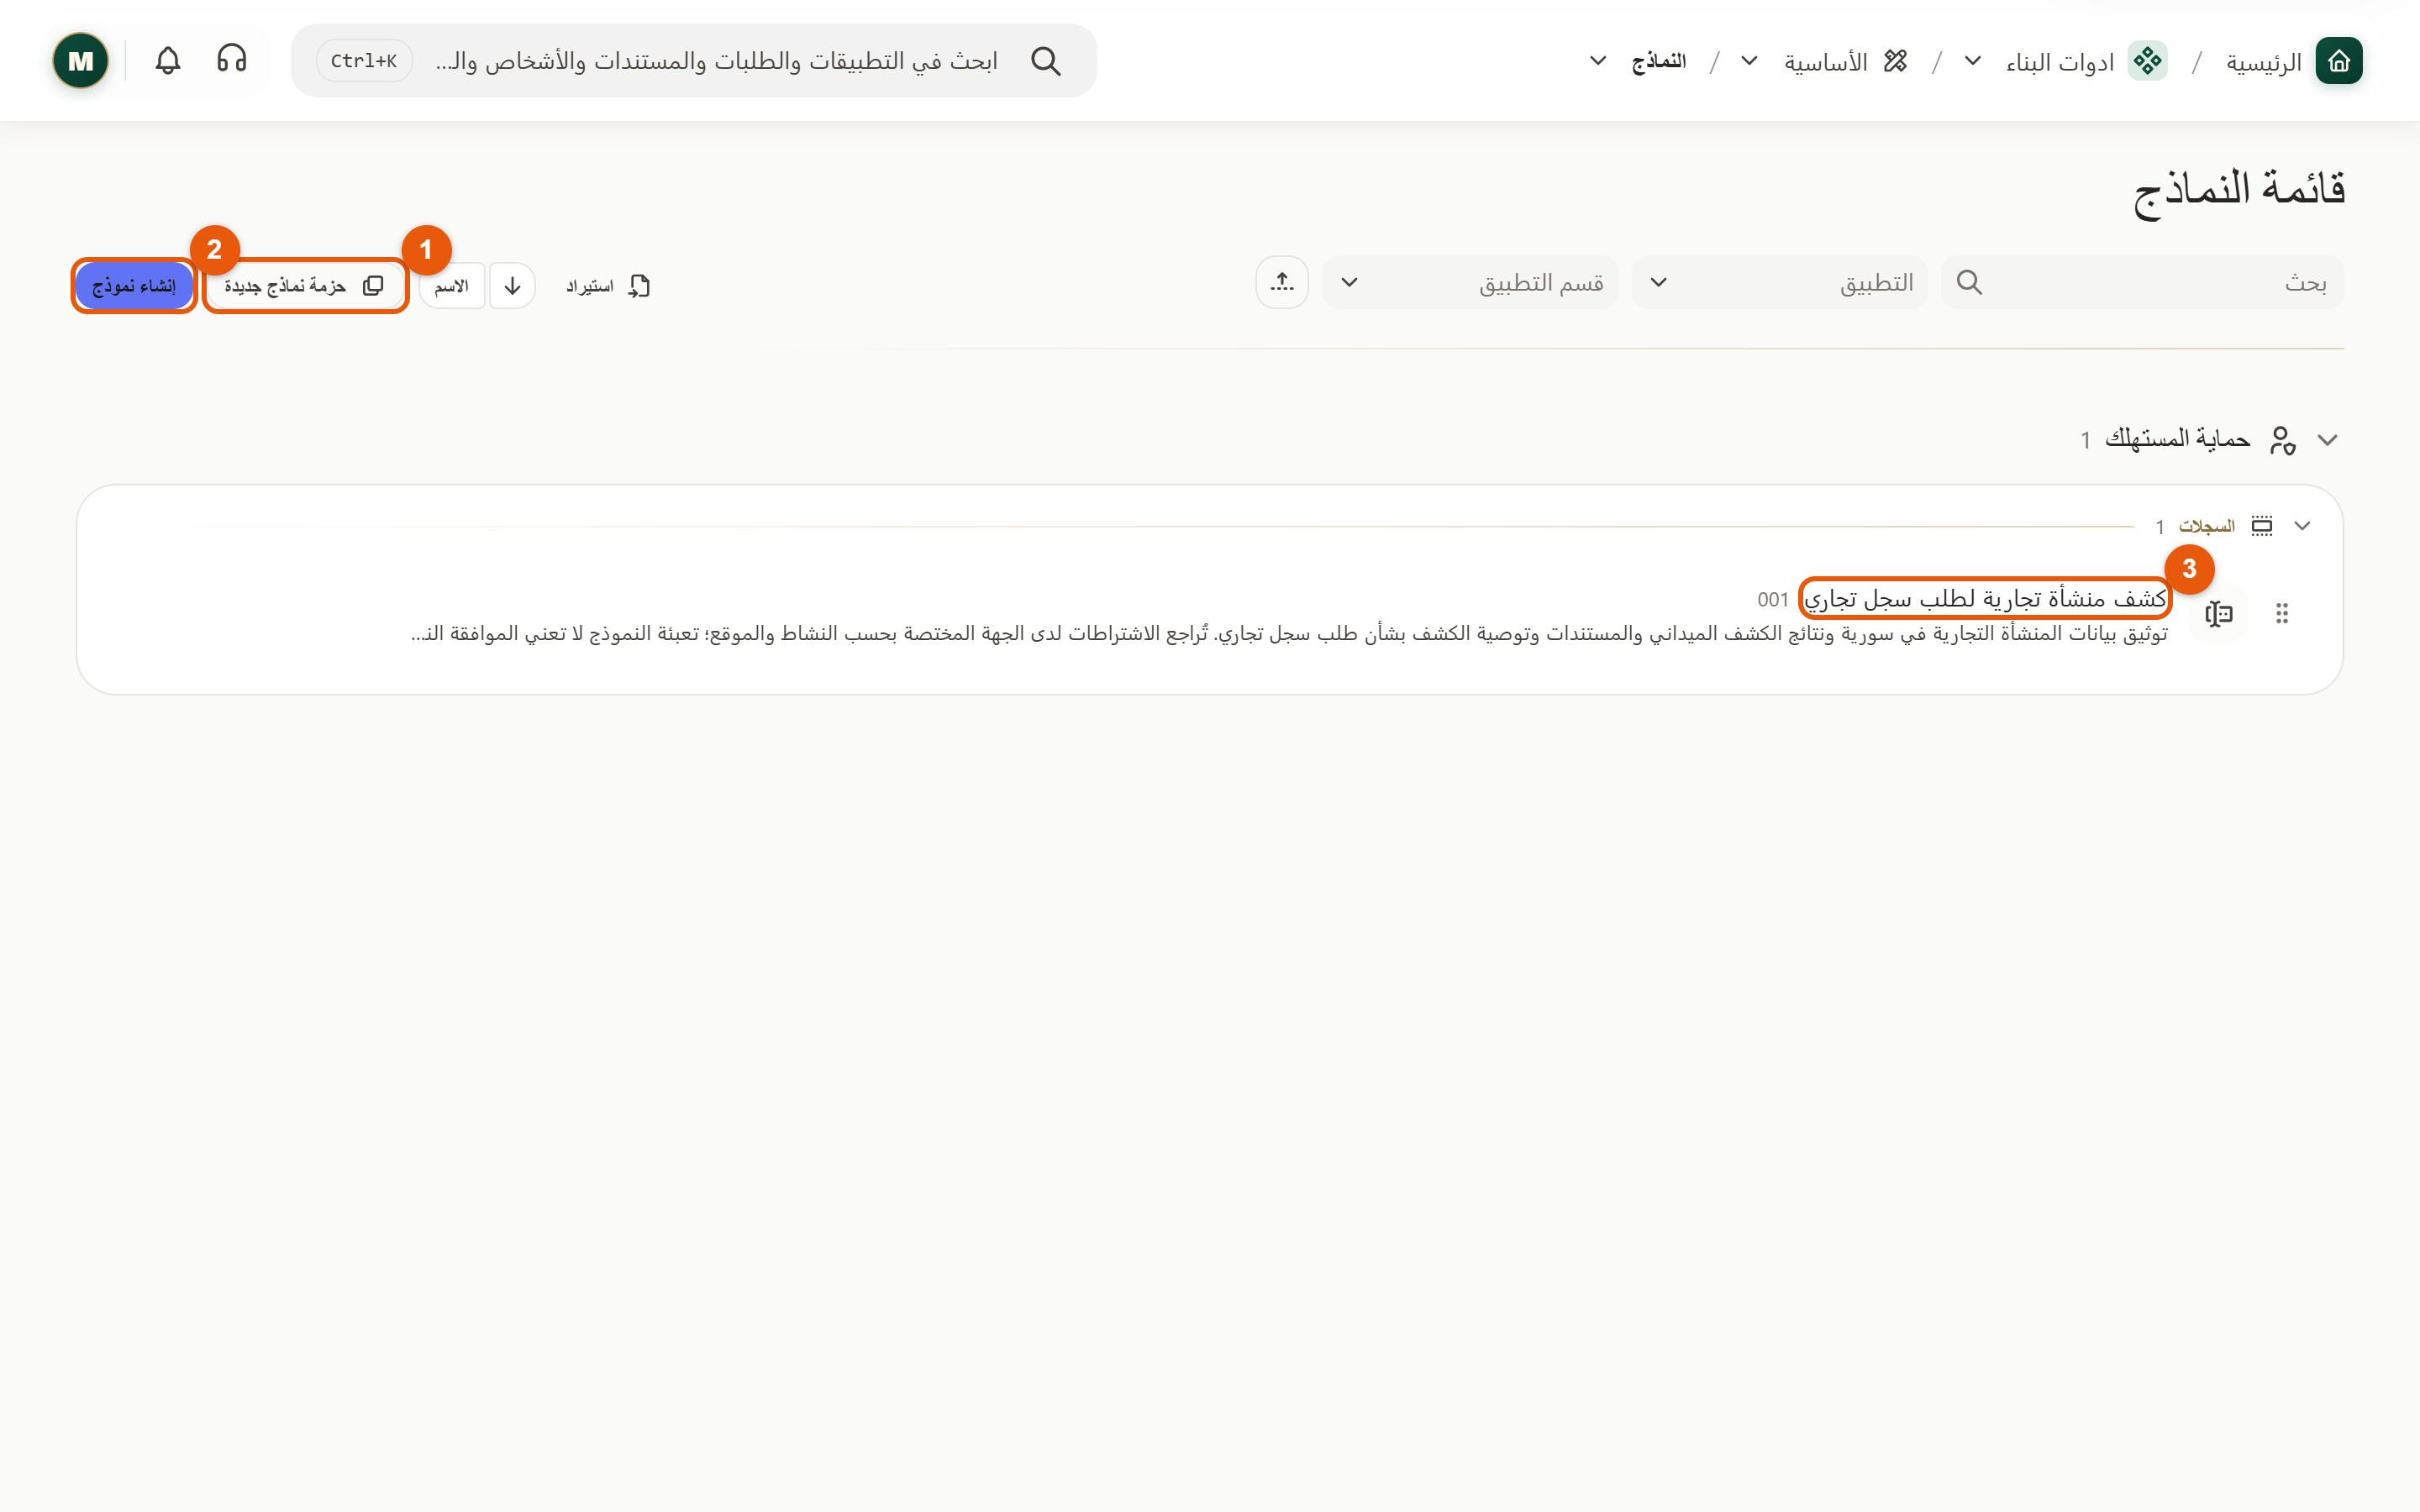
\includegraphics[width=0.95\linewidth]{assets/screens/forms-list.png}
\caption{النماذج والحزم في صفحة واحدة}
\label{fig:compare-forms-list}
\shotnote{تجمع «قائمة النماذج» النماذج وحزمها، فتبدأ منها أياً كان ما تبنيه. وتظهر الحزم في قسم خاص بعد إنشاء أول حزمة. ① «حزمة نماذج جديدة»: تنشئ حزمة تجمع نماذج منشورة. ② «إنشاء نموذج»: تنشئ نموذجاً واحداً. ③ بطاقة النموذج: تفتح منشئ النماذج.}
\end{figure}

\section{كل ما يسمى إجراء في كيان}
\label{sec:compare-procedures}

تظهر كلمة «إجراء» في أربعة أماكن مختلفة، وهذا أكثر ما يسبب الالتباس. فثلاثة منها تنفذ العمل، والرابع يوثّقه. ولا يغني أحدها عن الآخر؛ فبطاقة في الدليل لا تنقل طلباً، وأتمتة ناجحة لا تشرح للموظف سبب الخطوة.

\begin{rcnote}[مثال: مديرية الواحة]
توثّق المديرية إجراء الكشف في «دليل الإجراءات» ليعرفه كل موظف جديد. ويسير كل كشف فعلياً في مسار الطلب، وتتولى الأتمتة إنشاء مهمة المتابعة بعد الرفض.
\end{rcnote}

\begin{table}[H]
\centering
\caption{الأسماء الأربعة}
\label{tab:compare-procedures}
\begin{tabularx}{\linewidth}{R{3.8cm} Y}
\rcHeaderRow
\thh{الاسم في النظام} & \thh{ما هو؟ ومتى تستخدمه؟}\\
مسار الطلب & حالات الرد وموافقاته داخل نموذج واحد. استخدمه لقرار يخص الرد نفسه.\\
«الإجراءات الداخلية» & مسارات مؤتمتة تُبنى داخل كيان خطوة بعد خطوة، ولها «عمليات التشغيل» و«المتغيرات». وهي ميزة تجريبية.\\
«إجراءات التشغيل القياسية» & أتمتة بمحرك مستقل تربط كيان بخدمات أخرى من خلال «الاتصالات». وبعض شاشاتها بالإنجليزية حالياً.\\
«دليل الإجراءات» & بطاقات تشرح طريقة العمل، ولها مالك وخطوات وإصدارات، ويمكن البدء باستيراد دليل PDF.\\
\end{tabularx}
\end{table}

\begin{figure}[H]
\centering
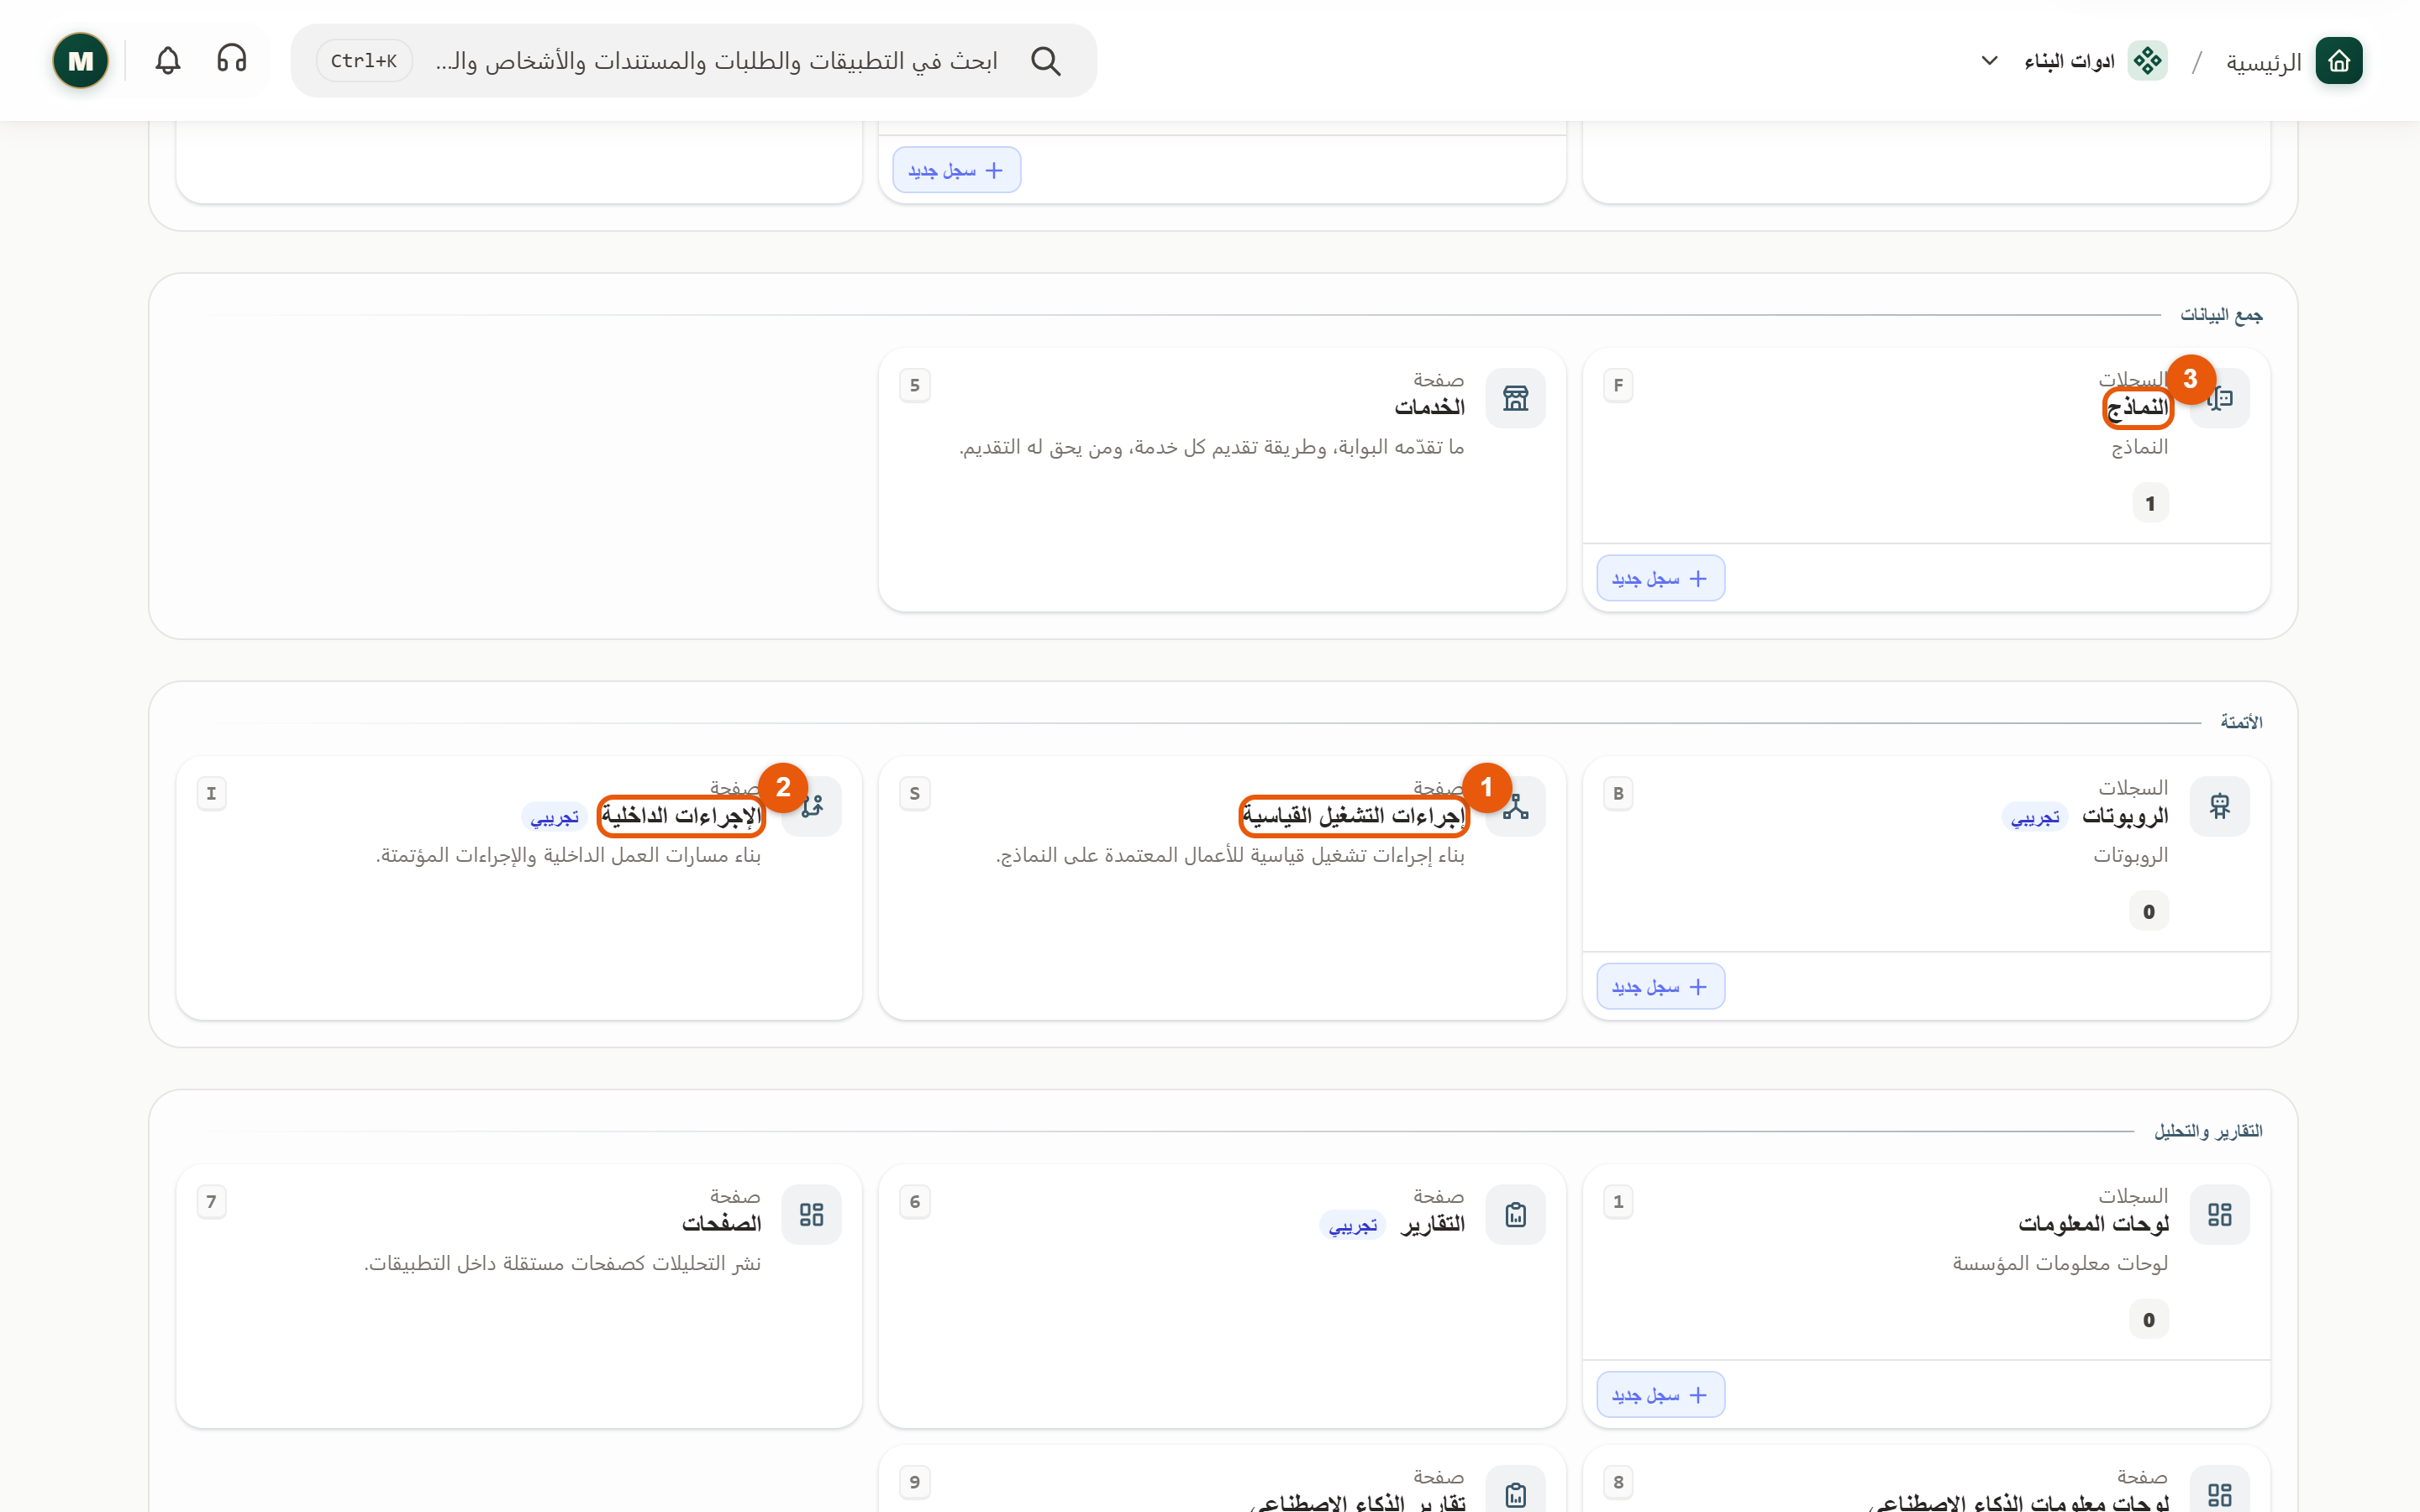
\includegraphics[width=0.95\linewidth]{assets/screens/tools-automation.png}
\caption{أدوات البناء: من أين تفتح كلاً منها}
\label{fig:compare-tools}
\shotnote{تقسّم «ادوات البناء» أدواتها بحسب الغرض، فتجد النماذج في «جمع البيانات» والأتمتة في قسمها. ① «إجراءات التشغيل القياسية». ② «الإجراءات الداخلية»: تحمل وسم «تجريبي». ③ «النماذج».}
\end{figure}

\begin{figure}[H]
\centering
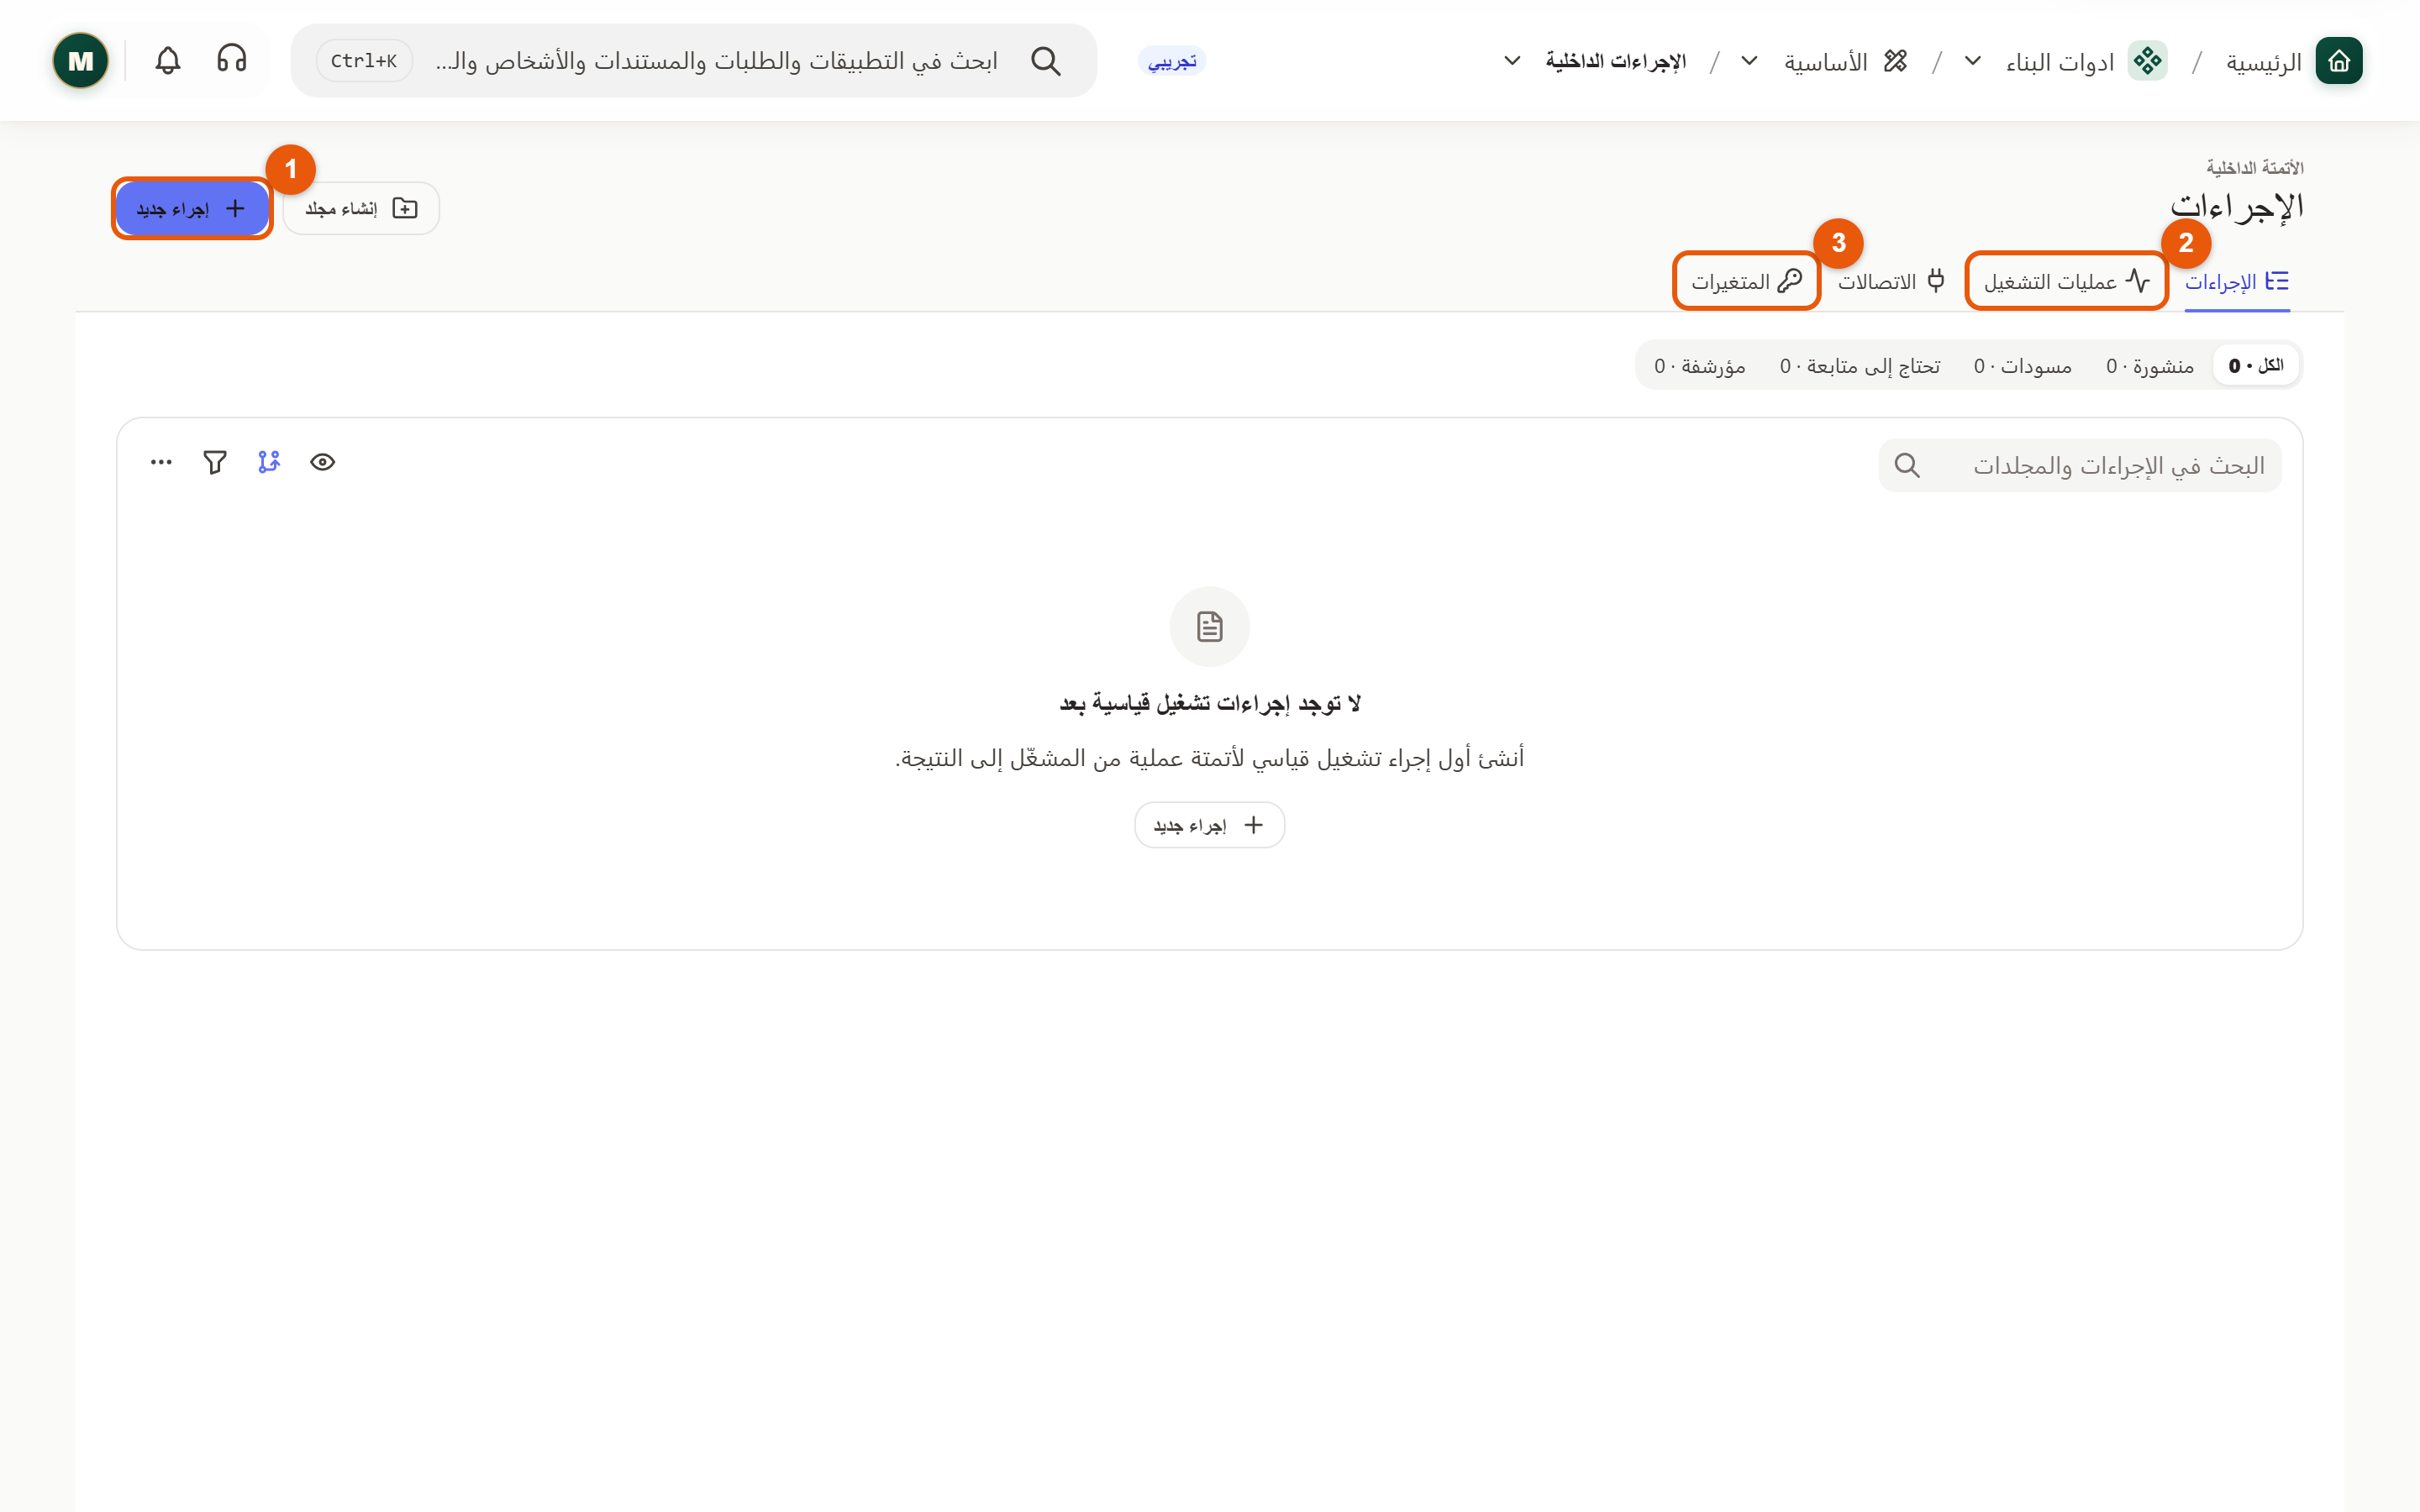
\includegraphics[width=0.95\linewidth]{assets/screens/internal-sop.png}
\caption{«الإجراءات الداخلية»}
\label{fig:compare-internal}
\shotnote{تعرض الصفحة كل إجراء مع حالته وآخر عمليات تشغيله، وهي فارغة هنا لأن المؤسسة لم تنشئ إجراءً بعد. ① «إجراء جديد»: يبدأ البناء. ② «عمليات التشغيل»: تبيّن ما نجح وما فشل، ومنها يبدأ التحقق بعد النشر. ③ «المتغيرات»: قيم يعاد استخدامها في الخطوات.}
\end{figure}

\begin{figure}[H]
\centering
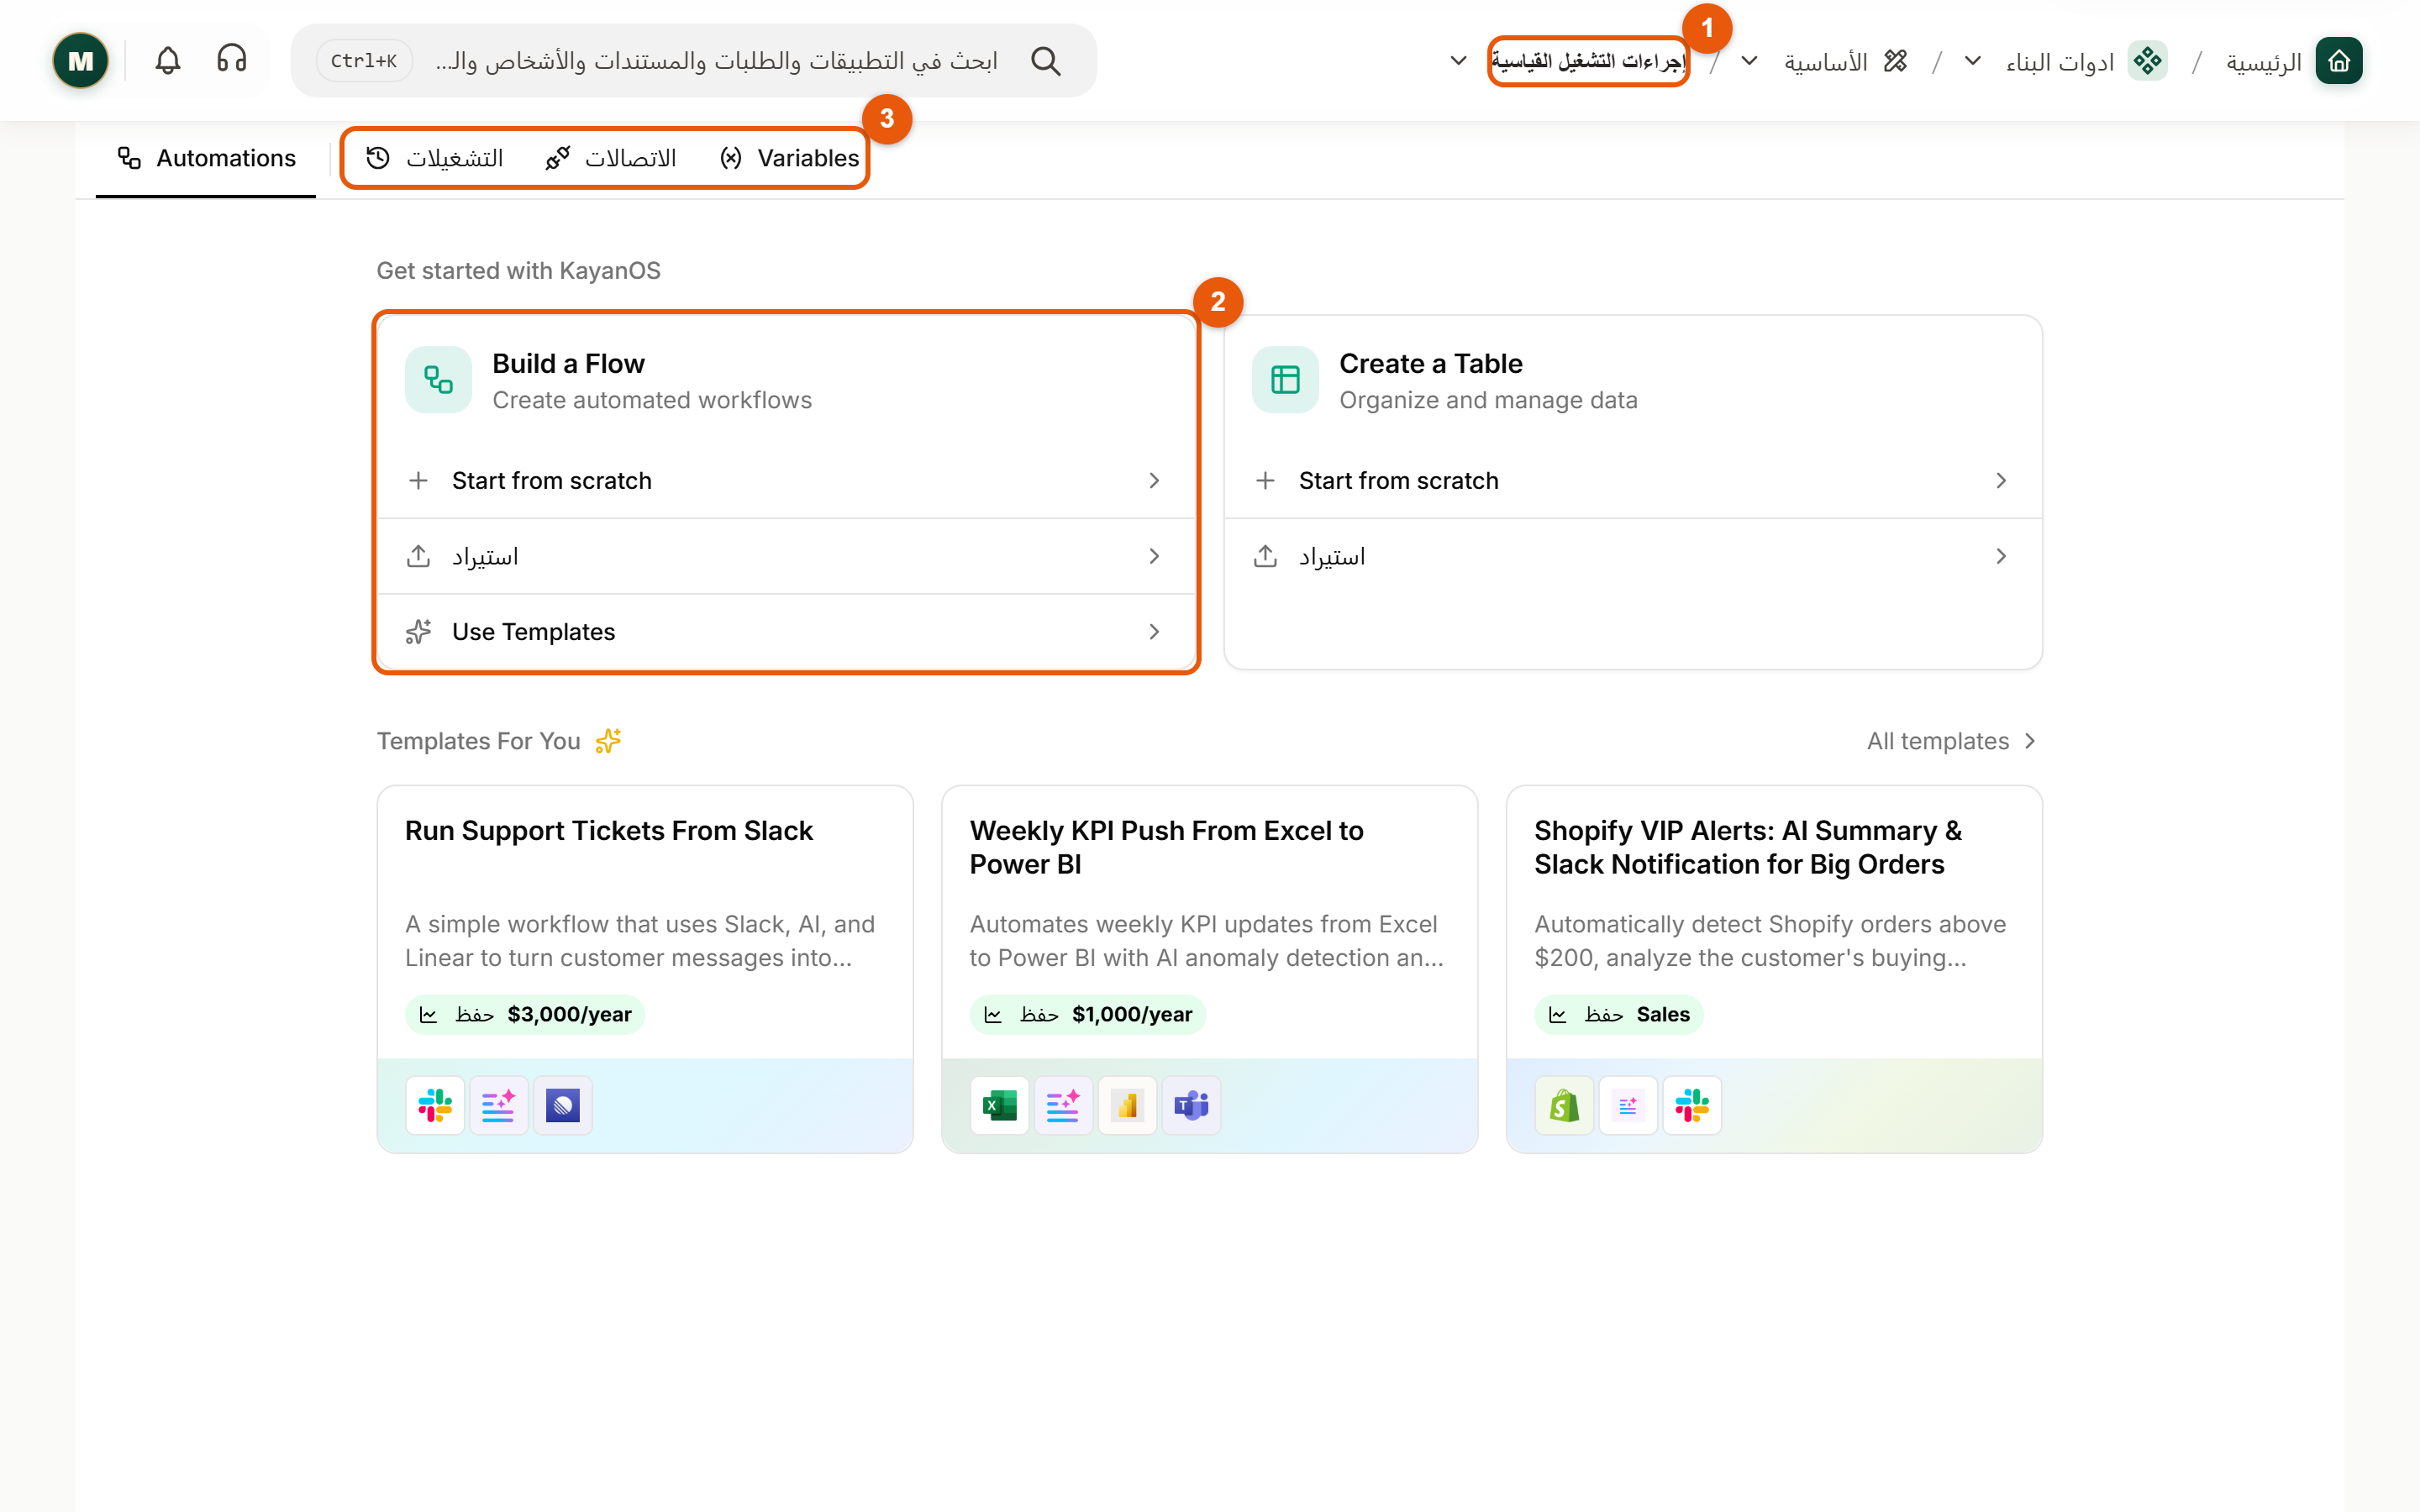
\includegraphics[width=0.95\linewidth]{assets/screens/sop-home.png}
\caption{«إجراءات التشغيل القياسية»}
\label{fig:compare-sop}
\shotnote{تفتح هذه الصفحة محرك الأتمتة داخل كيان، لذلك تظهر فيها عبارات بالإنجليزية. والقوالب المعروضة أمثلة عامة من المحرك، وليست من عملك. ① موقعك في أدوات البناء. ② «Build a Flow»: يبدأ أتمتة جديدة من الصفر أو من قالب. ③ التشغيلات والاتصالات والمتغيرات: تتابع منها ما جرى وما يربطه الإجراء.}
\end{figure}

\begin{figure}[H]
\centering
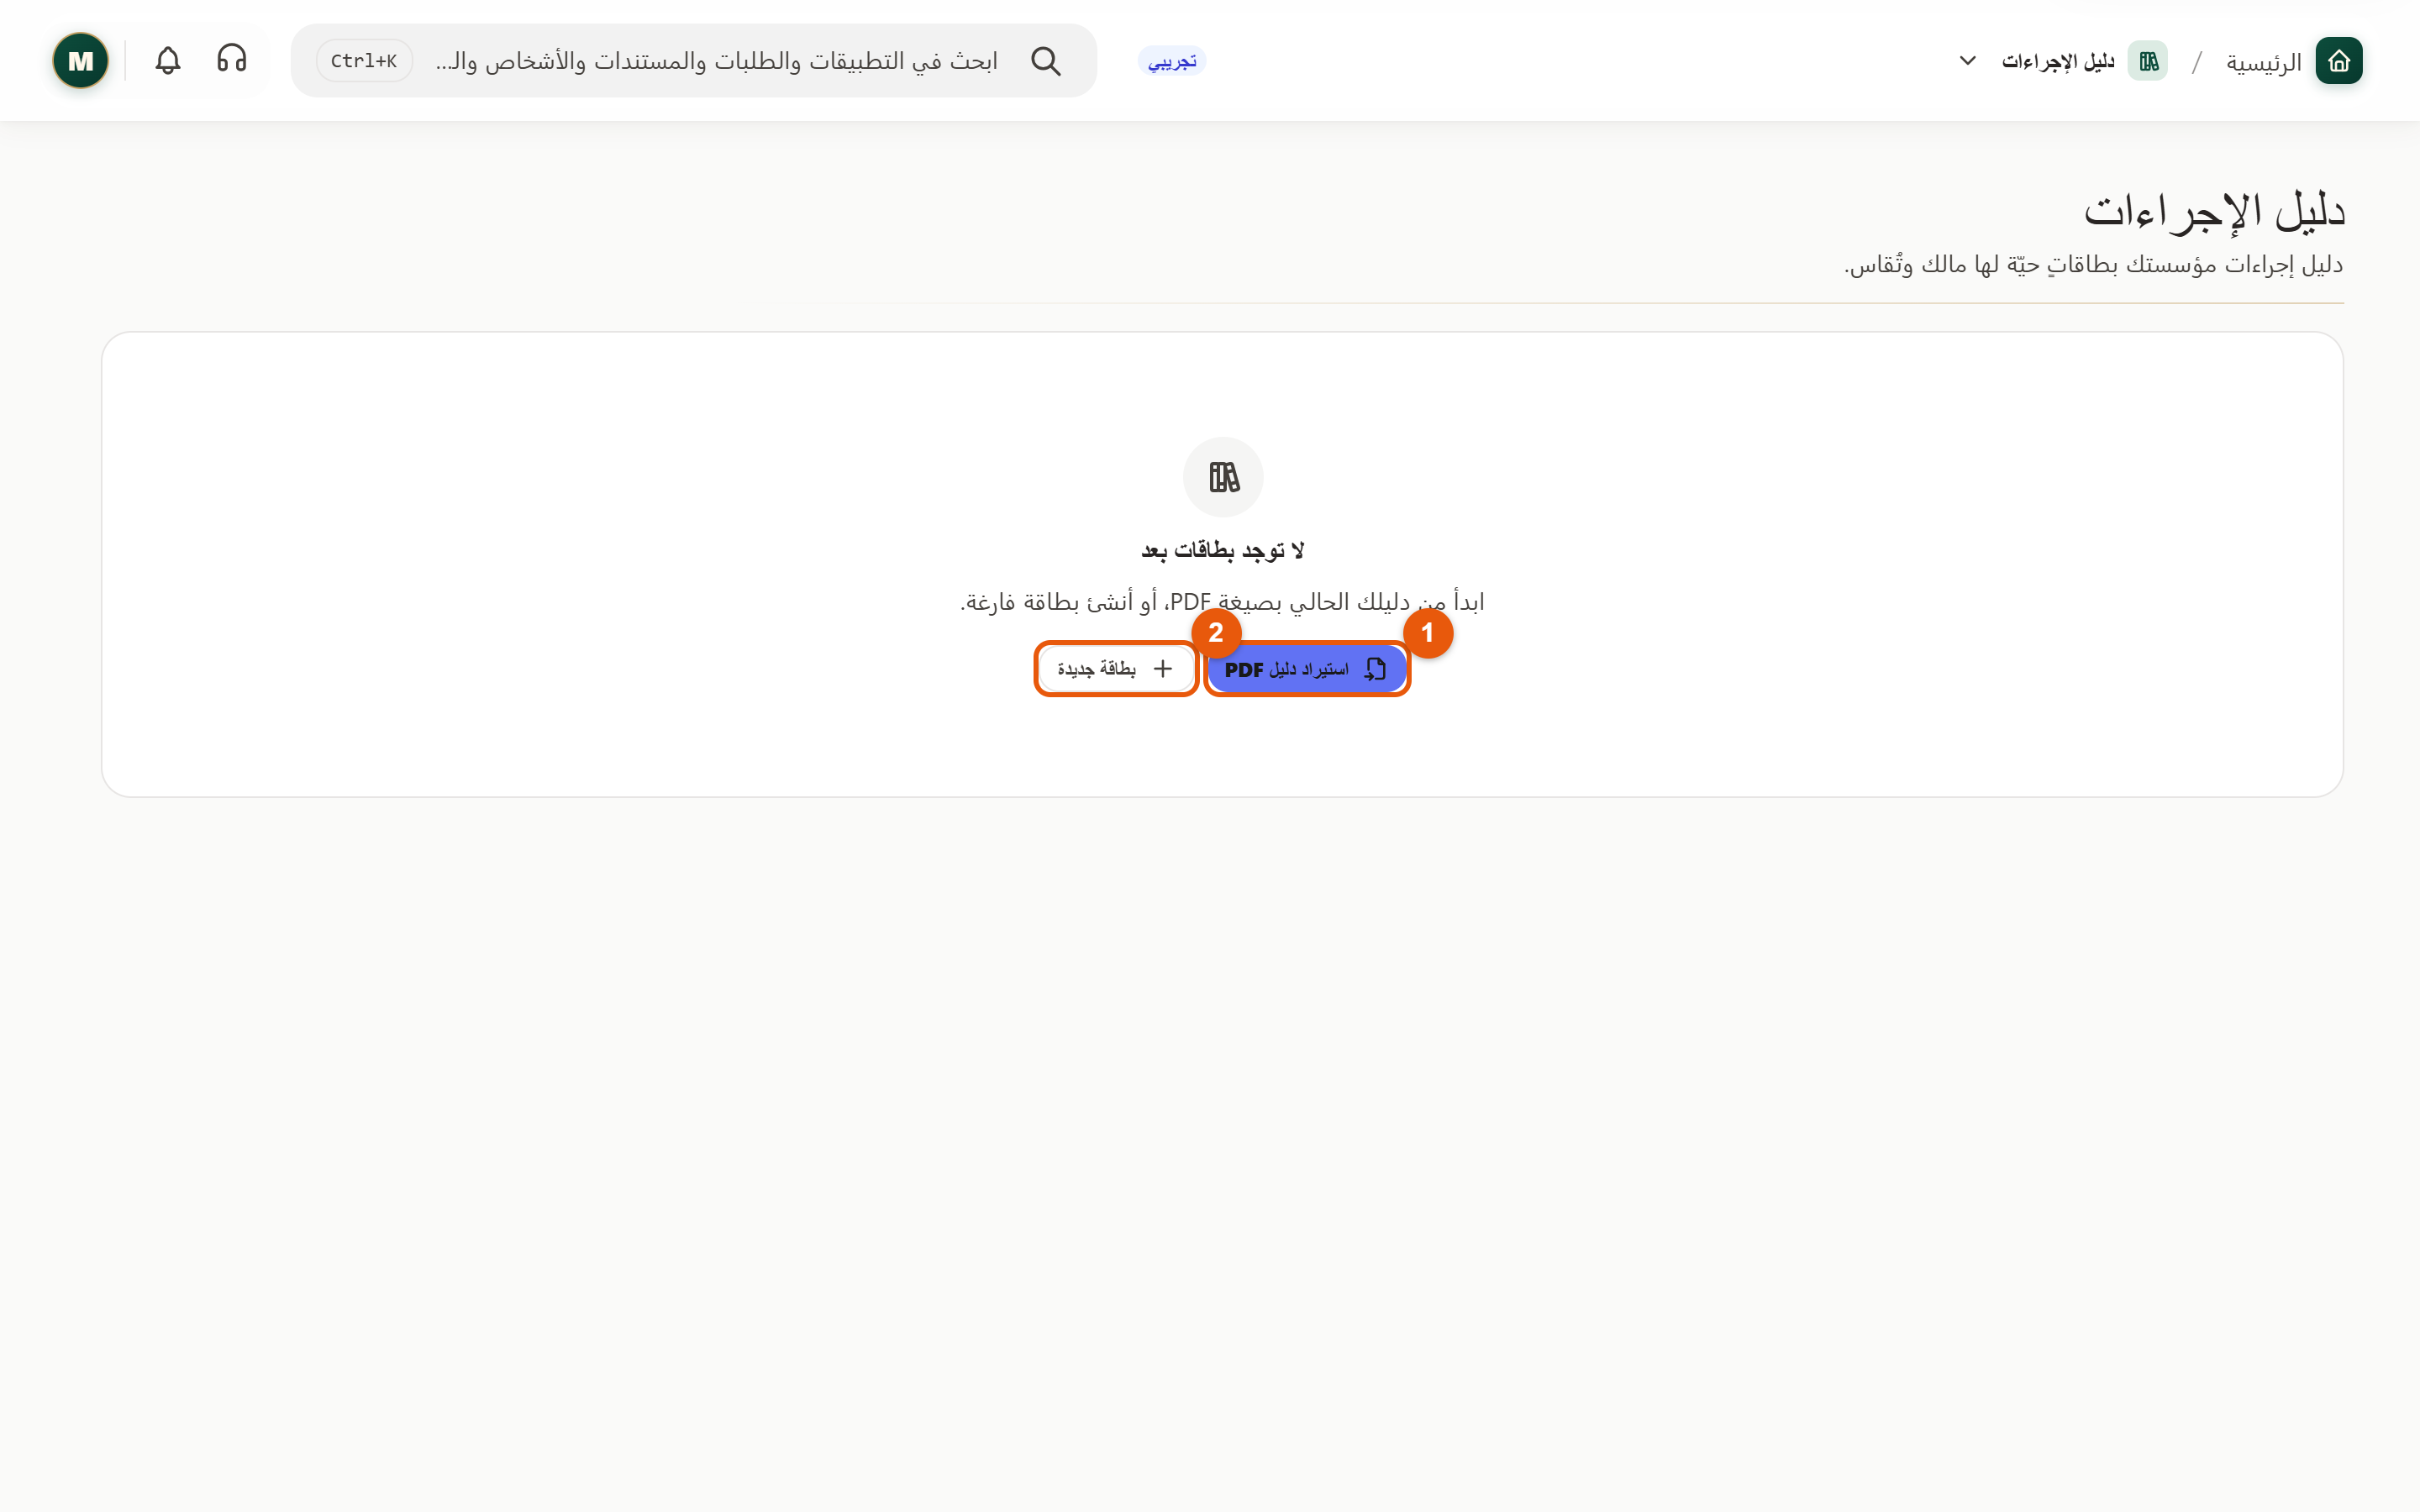
\includegraphics[width=0.95\linewidth]{assets/screens/procedures.png}
\caption{«دليل الإجراءات»}
\label{fig:compare-manual}
\shotnote{يحوّل الدليل المكتوب إلى بطاقات حيّة يملكها منصب محدد. وتبقى الصفحة فارغة حتى تضيف أول بطاقة. ① «استيراد دليل PDF»: يبدأ من دليلك الحالي. ② «بطاقة جديدة»: يكتب إجراءً واحداً من البداية.}
\end{figure}

\section{ابنِ حزمة نماذج}
\label{sec:compare-package}

تجمع حزمة النماذج نماذج منشورة في مهمة واحدة لكل سجل، وتسمى كل منها «وحدة». وتبقى لكل وحدة إجابتها ومراجعتها واعتمادها وكتابتها إلى السجلات، بينما تضيف الحزمة الترتيب والشروط والتقدم الموحّد.

استخدمها عندما يتكرر عمل من أكثر من نموذج على السجل نفسه. أما إذا كان لديك نموذج واحد، فلا تحتاج إلى حزمة؛ فخطة التكليف تكلّف به مباشرة.

\begin{rcnote}[مثال: مديرية الواحة]
تبني المديرية حزمة «جولة الالتزام الفصلية» عن سجلات «المنشآت التجارية». الوحدة الأولى هي الكشف. والوحدة الثانية هي متابعة المخالفات، ولا تُفتح إلا بعد قبول الكشف وإذا كانت هناك مخالفة. وإذا لم توجد مخالفة، تُتخطى المتابعة بعبارة «لا تنطبق» على هذا السجل.
\end{rcnote}

\begin{figure}[H]
\centering
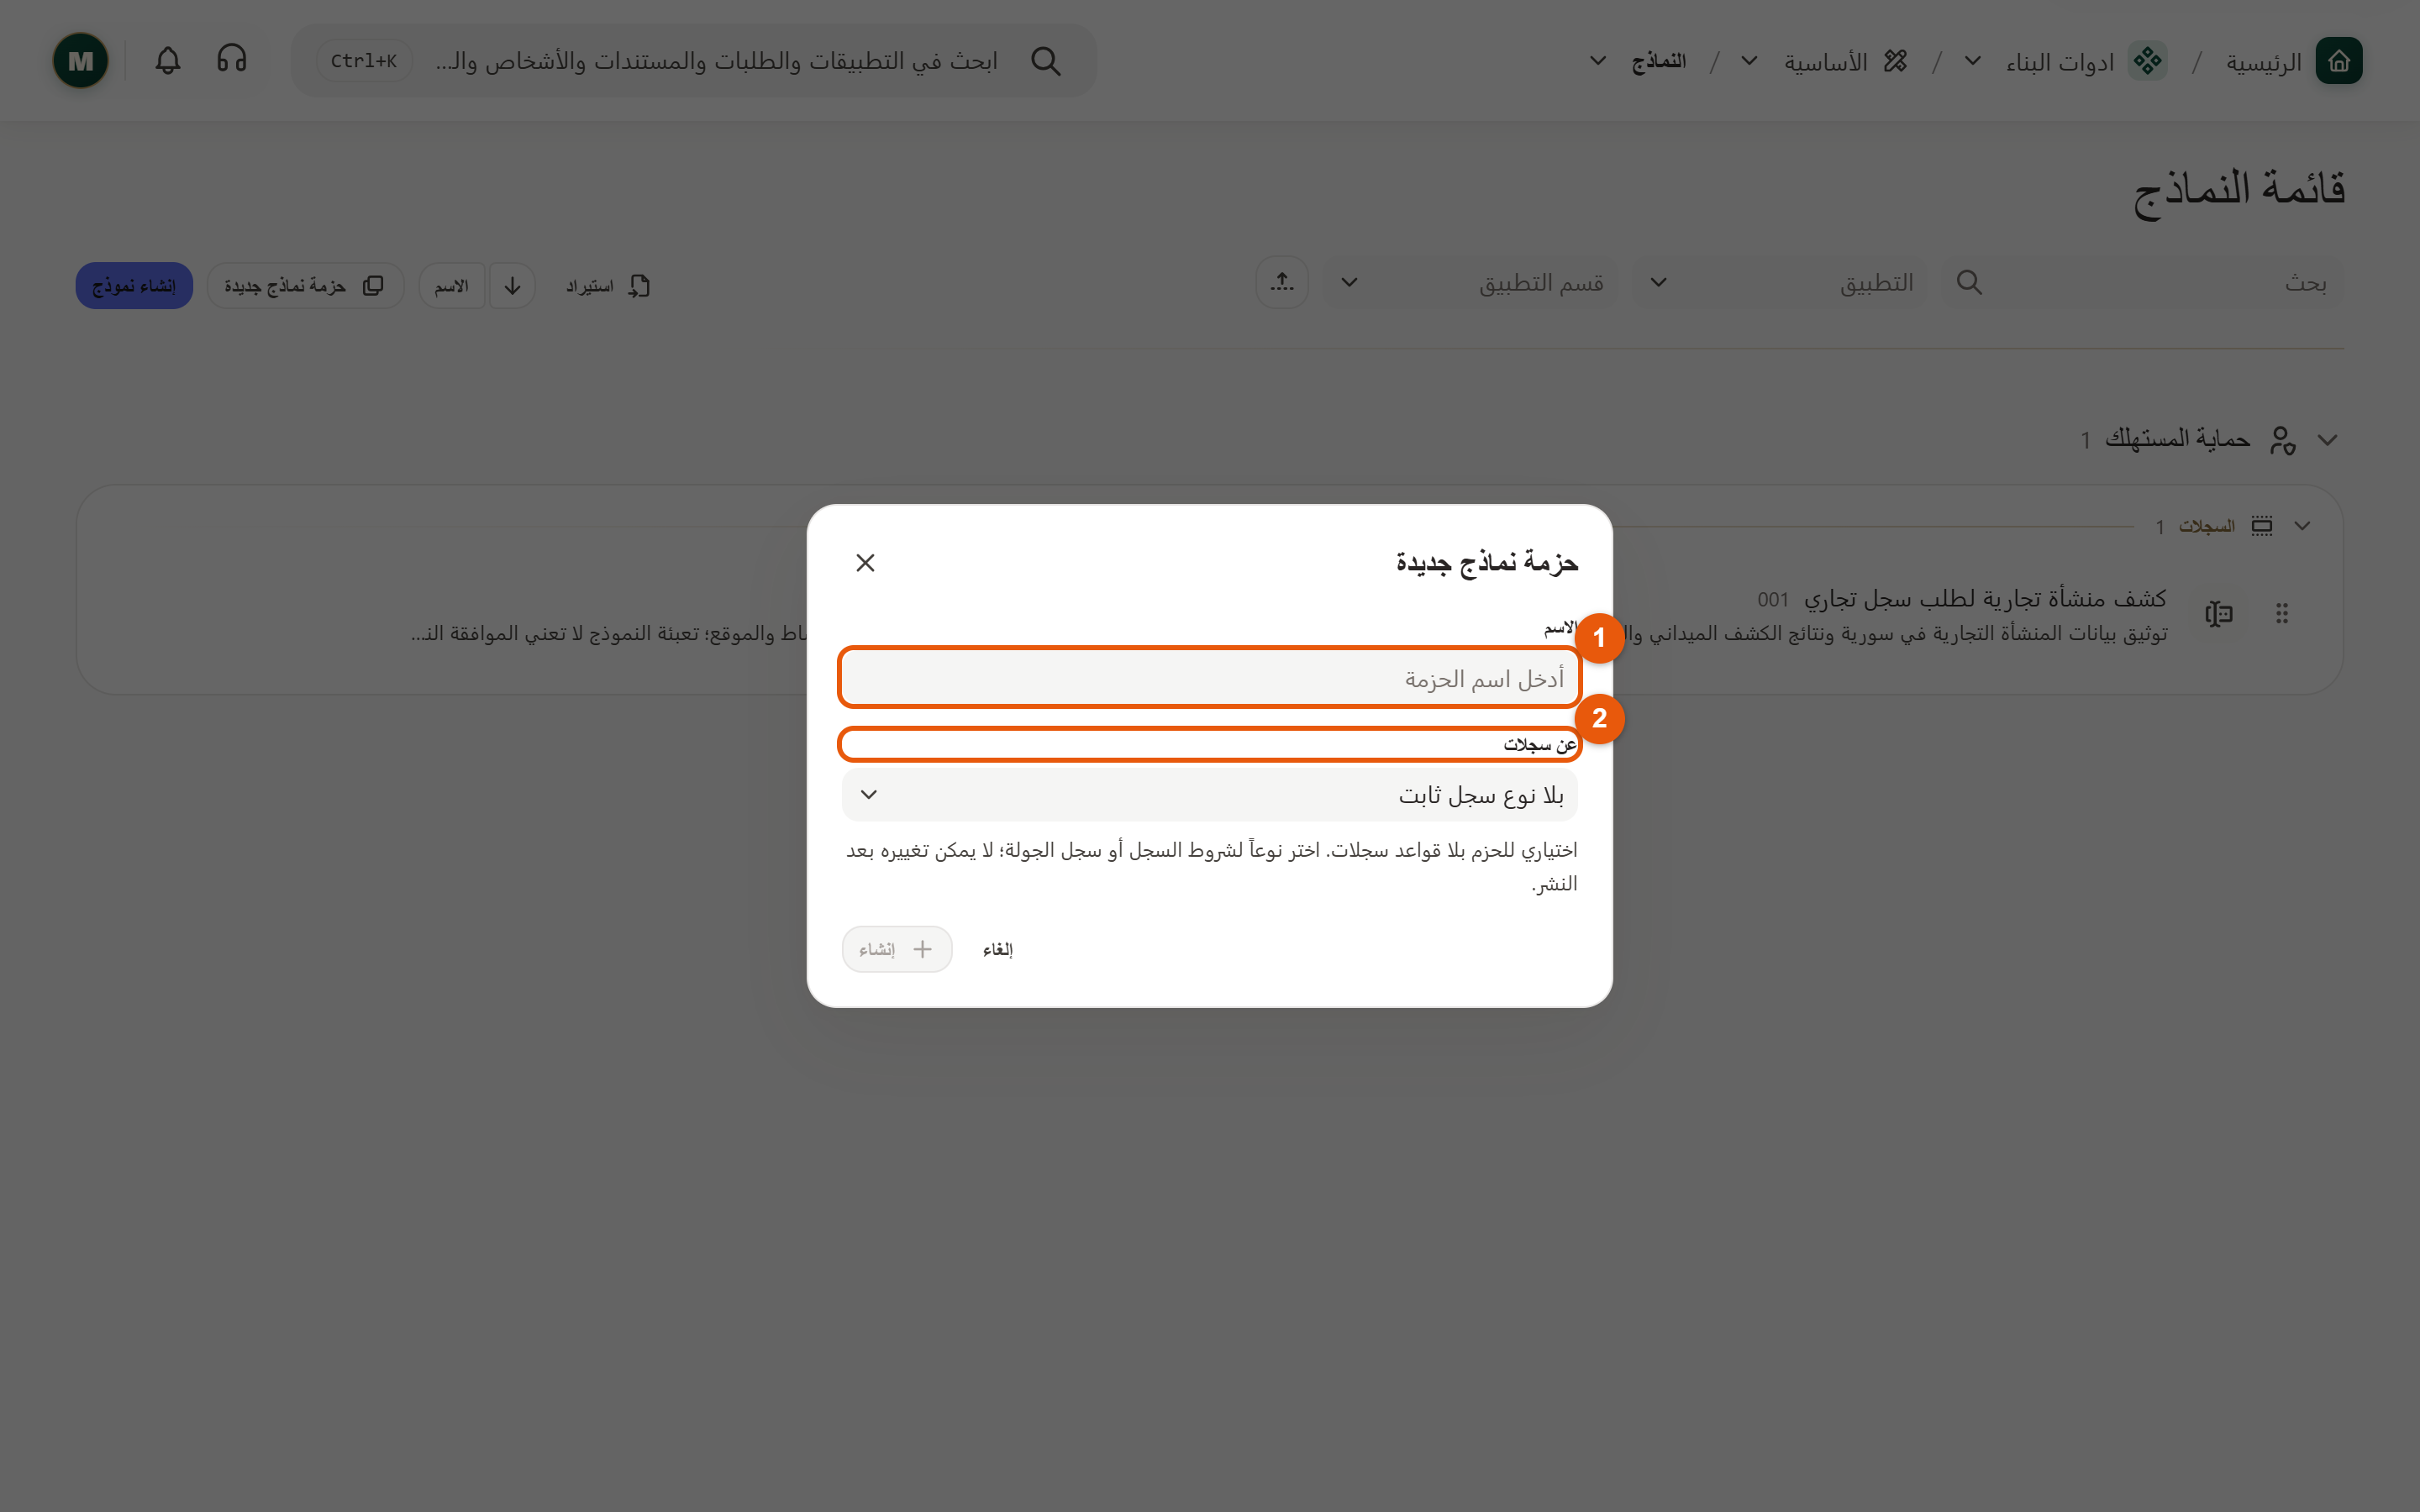
\includegraphics[width=0.62\linewidth]{assets/screens/package-new.png}
\caption{إنشاء الحزمة}
\label{fig:compare-package-new}
\shotnote{تطلب النافذة قرارين فقط، لكن الثاني يثبت بعد النشر. ① «الاسم»: اسم يعرفه الفريق. ② «عن سجلات»: اختر نوع السجلات إذا احتجت إلى شروط تقرأ السجل أو إلى سجل الجولة؛ فلا يمكن تغييره بعد النشر.}
\end{figure}

\begin{figure}[H]
\centering
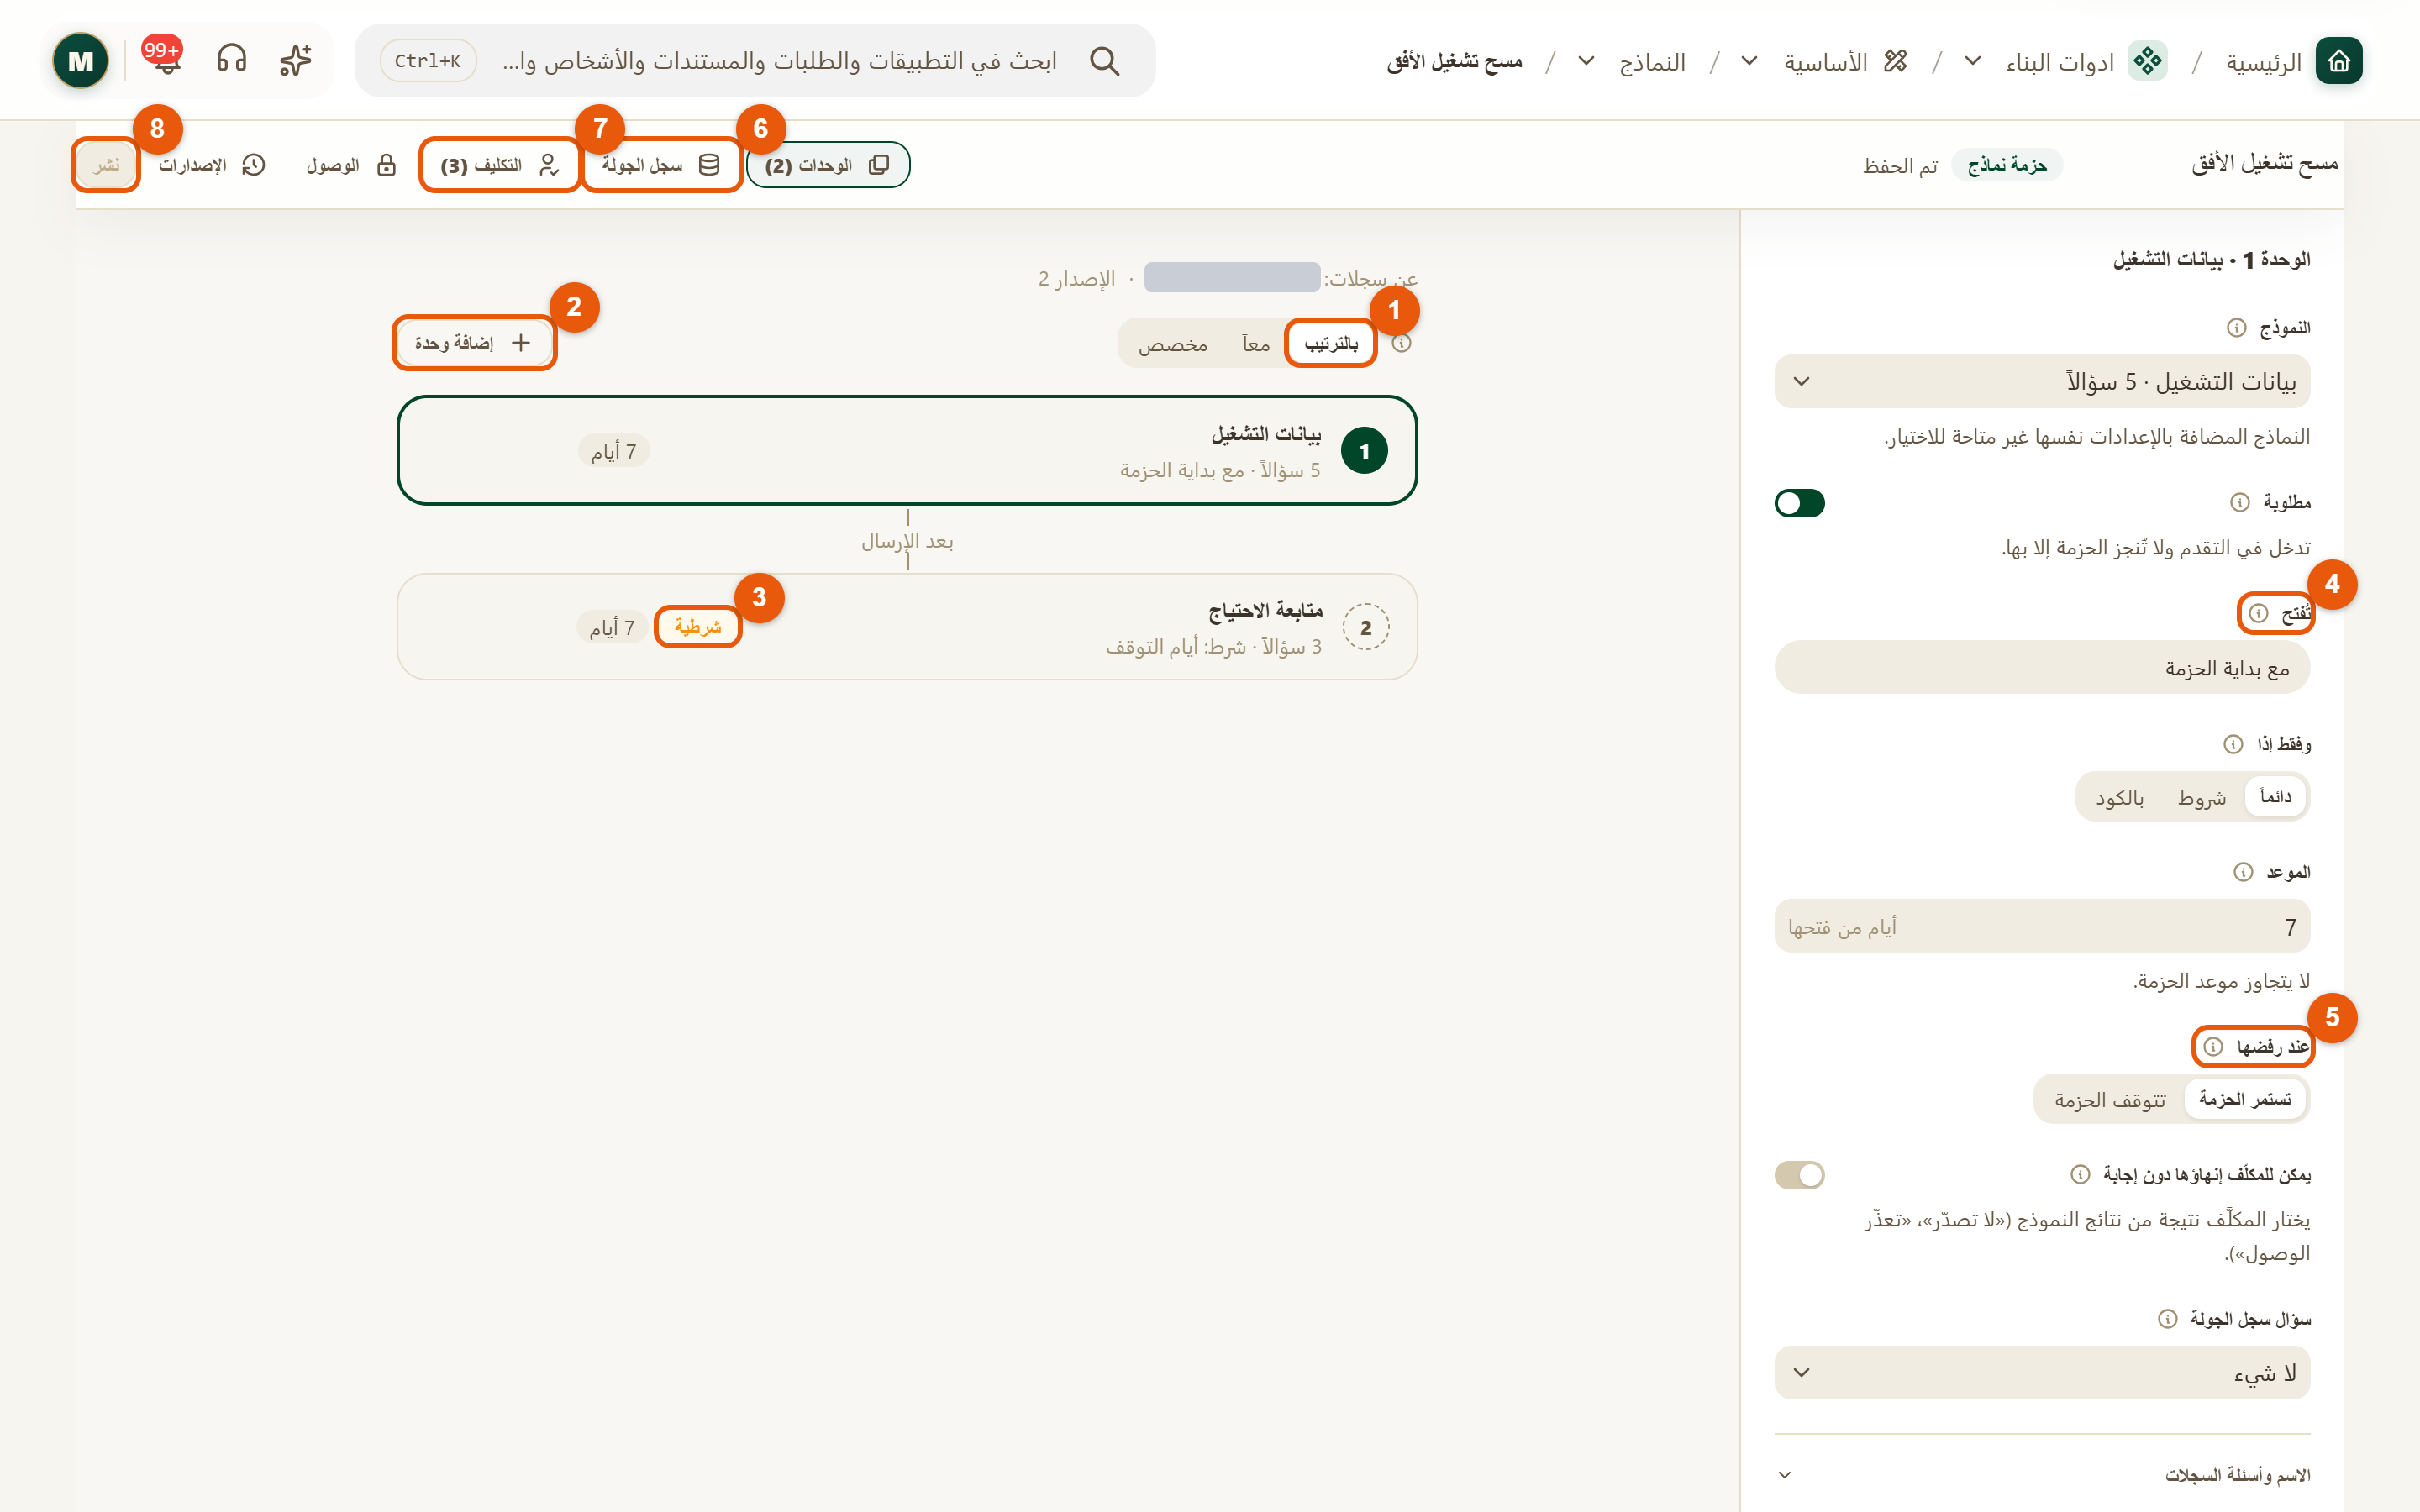
\includegraphics[width=0.95\linewidth]{assets/screens/package-editor.png}
\caption{محرر الحزمة}
\label{fig:compare-package-editor}
\shotnote{تعرض اللوحة الوحدات بترتيبها، ويعرض الشريط الجانبي إعداد الوحدة المحددة. والحزمة في الصورة مثال تجريبي بوحدتين، وليست من مثال الواحة. ① «بالترتيب»: كيف تُفتح الوحدات؛ والخياران الآخران «معاً» و«مخصص». ② «إضافة وحدة»: تضيف نموذجاً منشوراً. ③ «شرطية»: وحدة لا تُفتح إلا بتحقق شرطها. ④ «تُفتح»: متى تبدأ الوحدة. ⑤ «عند رفضها»: هل تستمر الحزمة أم تتوقف. ⑥ «سجل الجولة»: سجل واحد لكل سجل في كل جولة. ⑦ «التكليف»: الخطط التي تطلق الحزمة. ⑧ «نشر»: لا يمكن للخطط التكليف بالحزمة قبله.}
\end{figure}

\begin{table}[H]
\centering
\caption{إعدادات الوحدة}
\label{tab:compare-module}
\begin{tabularx}{\linewidth}{R{3.6cm} Y}
\rcHeaderRow
\thh{الإعداد} & \thh{ما يقرره}\\
«مطلوبة» & تدخل في التقدم، ولا تُنجز الحزمة إلا بها.\\
«تُفتح» & «مع بداية الحزمة»، أو «بعد وحدات سابقة» عند إرسالها أو قبولها.\\
«وفقط إذا» & شرط إضافي: «دائماً» أو «شروط» أو «بالكود».\\
«إن لم يتحقق» & تُتخطى الوحدة «لا تنطبق»، أو «تبقى بانتظار تحققه».\\
«الموعد» & أيام من فتح الوحدة، ولا يتجاوز موعد الحزمة.\\
«عند رفضها» & «تستمر الحزمة» أو «تتوقف الحزمة».\\
«يمكن للمكلّف إنهاؤها دون إجابة» & يختار المكلَّف نتيجة من نتائج النموذج، مثل «تعذّر الوصول».\\
\end{tabularx}
\end{table}

\subsection{خطوات العمل والتحقق}
\begin{enumerate}
\item تأكد من نشر كل نموذج ستضيفه؛ فالوحدة لا تقبل نموذجاً غير منشور.
\item افتح «ادوات البناء» ← «النماذج»، واضغط «حزمة نماذج جديدة».
\item اكتب «الاسم»، واختر في «عن سجلات» نوع السجلات إن احتجته، ثم اضغط «إنشاء».
\item اضغط «إضافة وحدة»، وأضف النماذج بالترتيب.
\item حدّد الوحدة الثانية، واضبط «تُفتح» و«وفقط إذا» و«إن لم يتحقق».
\item اضغط «نشر».
\end{enumerate}

\textbf{تحقق:} يجب أن تظهر الحزمة في قسم «حزم النماذج» مع عدد الوحدات ورقم الإصدار. وإذا ظهرت «غير منشورة»، فعالج المشكلات المعروضة في المحرر ثم انشر من جديد.

\begin{table}[H]
\centering
\caption{رسائل قد تظهر قبل النشر}
\label{tab:compare-package-errors}
\begin{tabularx}{\linewidth}{R{6.2cm} Y}
\rcHeaderRow
\thh{الرسالة} & \thh{ما تفعله}\\
«نموذج إحدى الوحدات غير منشور.» & انشر النموذج، ثم عد إلى الحزمة.\\
«يجب أن تُفتح وحدة واحدة مع بداية الحزمة.» & اجعل «تُفتح» في الوحدة الأولى «مع بداية الحزمة».\\
«شرط يقرأ سجل الحزمة: اختر نوع سجلاتها من «الوصول».» & افتح «الوصول» واختر «عن سجلات».\\
\end{tabularx}
\end{table}

\section{أطلق العمل بخطة تكليف}
\label{sec:compare-plans}

الحزمة والنموذج تصميم فقط، ولا يصل شيء إلى الفريق حتى تطلق خطة. فالخطة تحدد ما يُعبّأ، وعن أي سجلات، ومن يعبّئه، وتتابع كل جولة. وكل تكليف مهمة واحدة، تضم وحدات الحزمة إن كان التكليف بحزمة.

\begin{rcnote}[مثال: مديرية الواحة]
ينشئ خالد خطة «جولة الربع الأخير» من حزمة «جولة الالتزام الفصلية»، ويختار منشآت «المزة»، ويوزعها على الباحثين. فتظهر لليلى مهمة لكل منشأة، ويتابع خالد الإنجاز والمتأخر من صفحة الخطة.
\end{rcnote}

\begin{figure}[H]
\centering
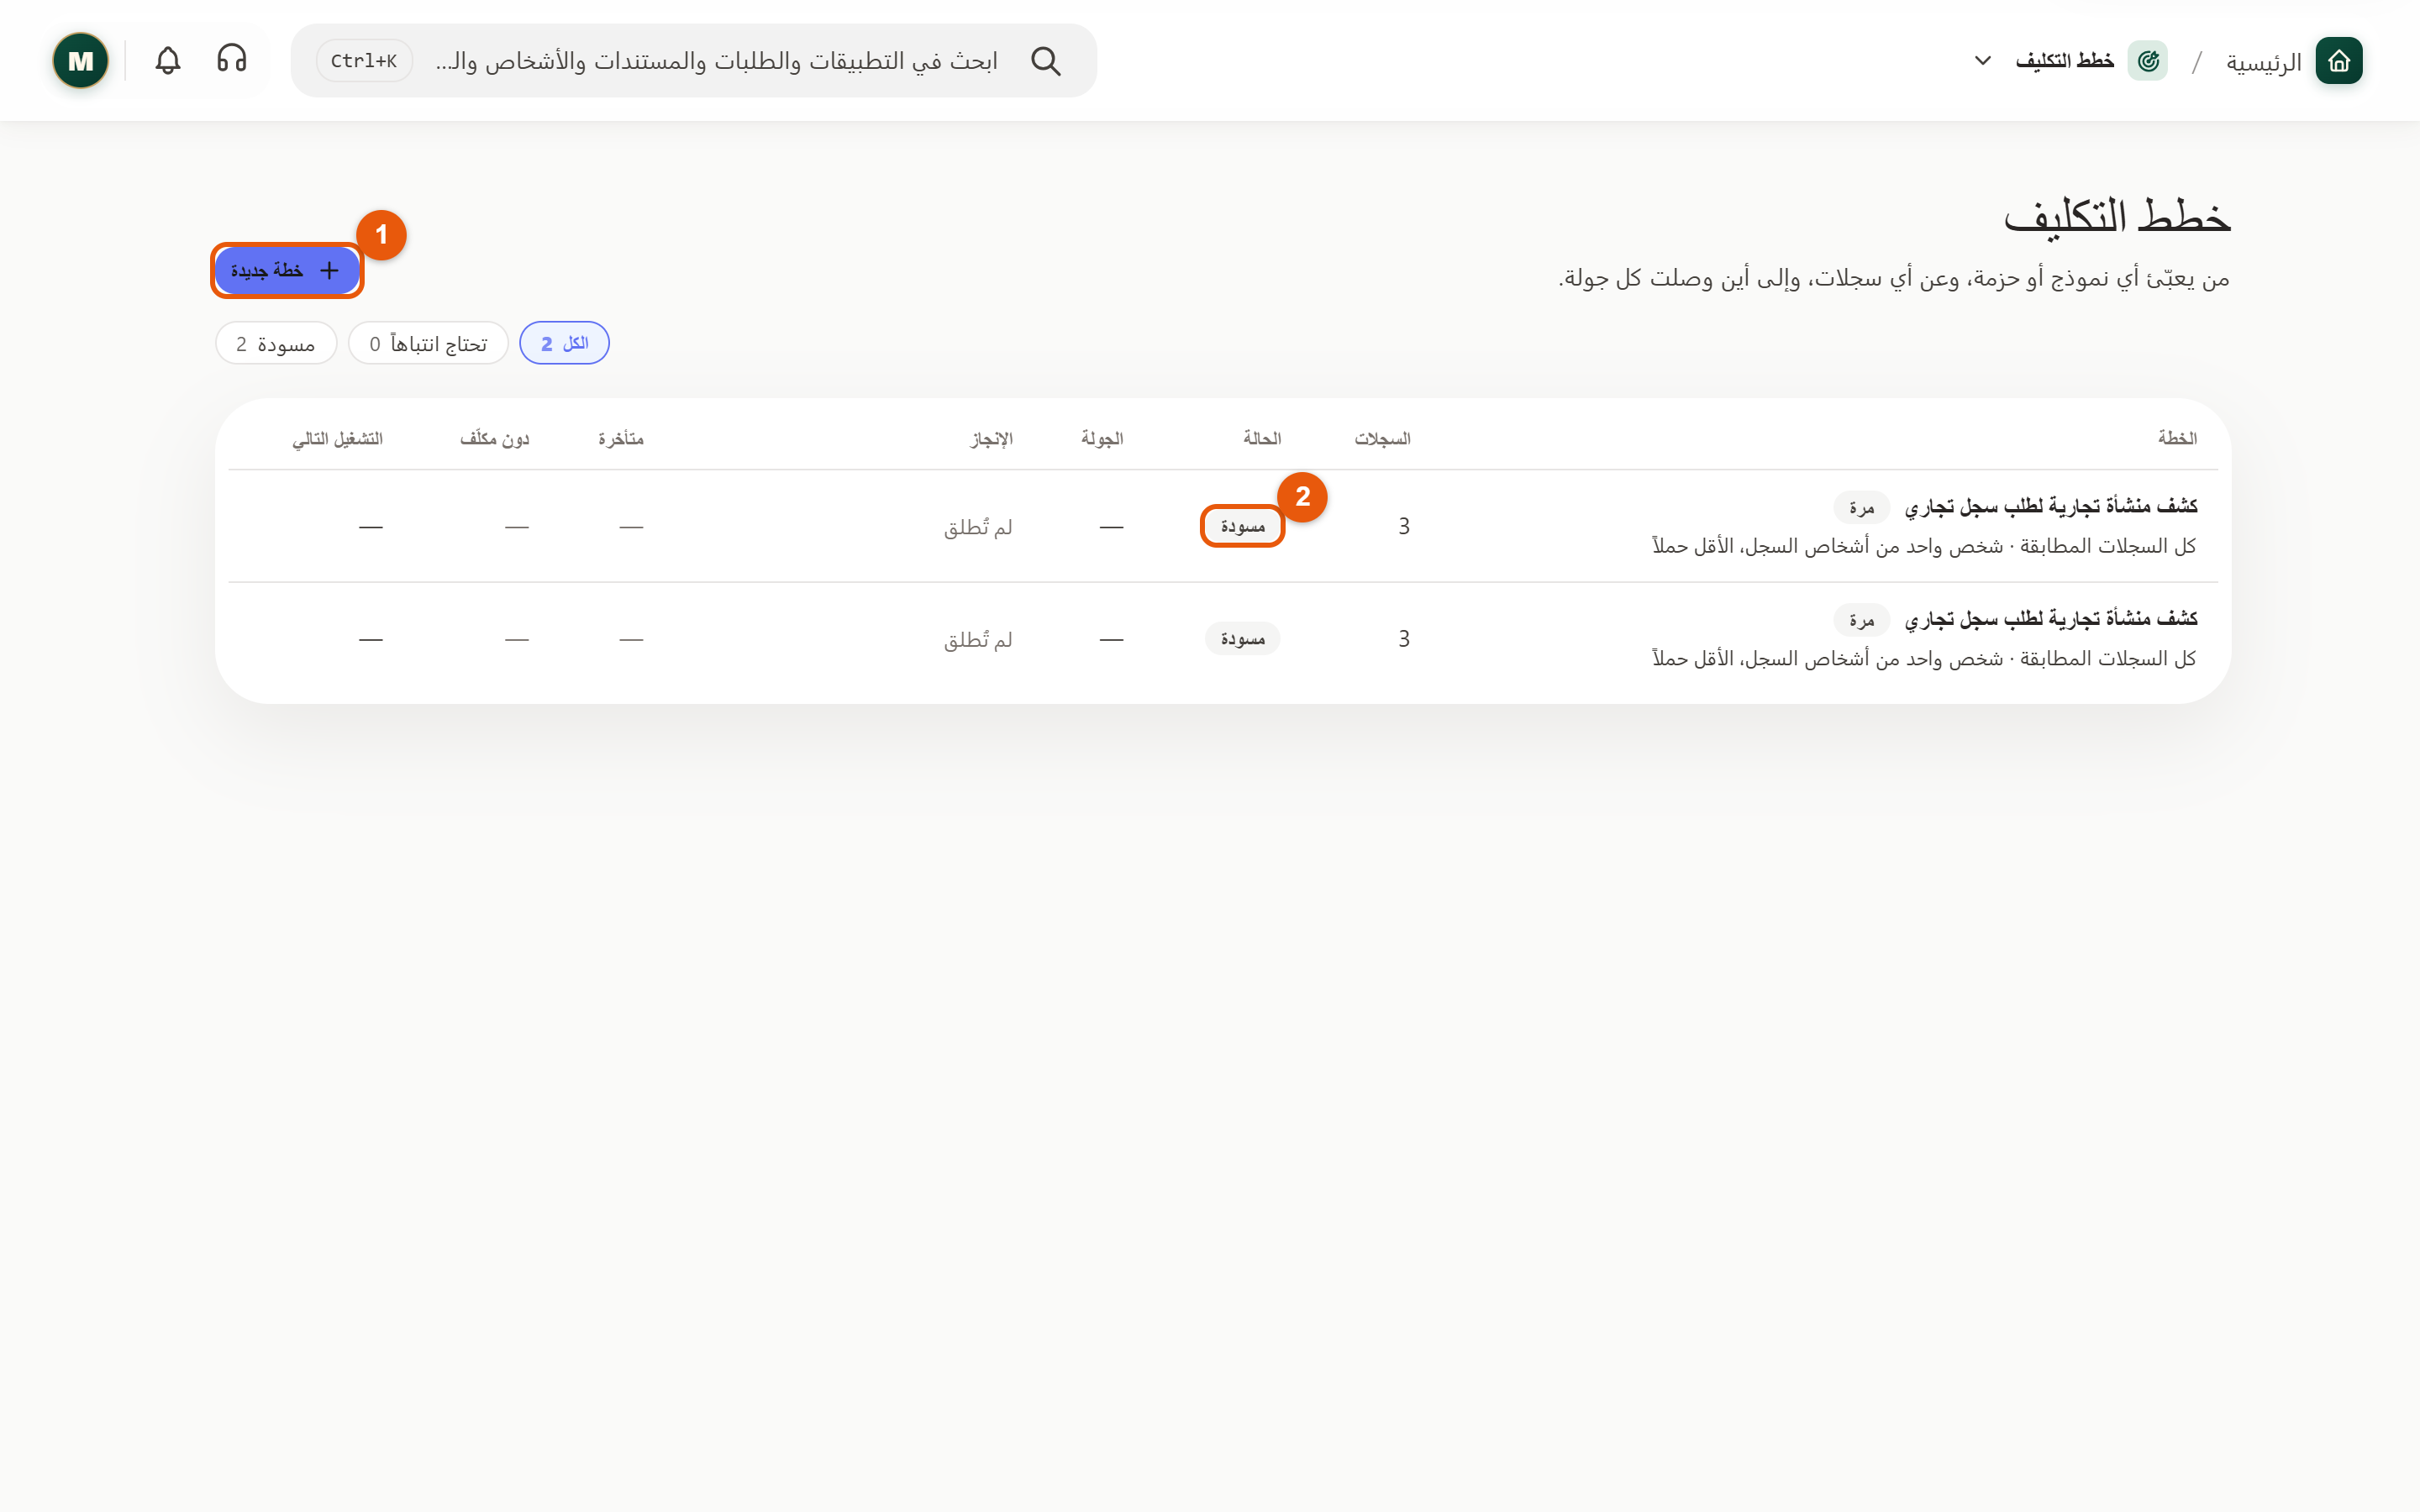
\includegraphics[width=0.95\linewidth]{assets/screens/plans-list.png}
\caption{«خطط التكليف»}
\label{fig:compare-plans}
\shotnote{تعرض الصفحة كل خطة مع سجلاتها وحالتها وجولتها وإنجازها. والخطتان في الصورة مسودتان، لذلك لم يصل منهما أي تكليف. ① «خطة جديدة». ② «مسودة»: الخطة لم تُطلق بعد، حتى لو كانت سجلاتها محددة.}
\end{figure}

\subsection{خطوات العمل والتحقق}
\begin{enumerate}
\item افتح «خطط التكليف»، واضغط «خطة جديدة»، أو ابدأ من «التكليف» داخل الحزمة.
\item سمِّ الخطة باسم يدل على الجولة، حتى لا تتشابه الخطط في القائمة.
\item حدّد السجلات والأشخاص، ثم أطلق الخطة.
\end{enumerate}

\textbf{تحقق:} ادخل بحساب أحد المكلَّفين، وافتح «تكليفات مطلوبة منك» من الصفحة الرئيسية. يجب أن ترى مهمة واحدة لكل سجل. وإذا بقيت حالة الخطة «مسودة»، فلم تُطلق بعد ولن يصل إليهم شيء.
